%%% Foaie de sumar — document de sine statator, doua pagini.
%%% Se compileaza separat: pdflatex rezumat.tex
\documentclass[11pt,a4paper]{article}

\usepackage[T1]{fontenc}
\usepackage[utf8]{inputenc}
\usepackage[romanian]{babel}
\usepackage{times}
\usepackage{amsmath,amssymb}
\usepackage{geometry}
\usepackage{titlesec}
\usepackage{enumitem}
\usepackage{tikz}
\usetikzlibrary{positioning,arrows.meta,fit,calc,shapes.geometric,backgrounds}

\geometry{a4paper, total={170mm,252mm}, left=20mm, top=20mm}
\setlist{noitemsep,topsep=2pt,leftmargin=5mm}
\titlespacing*{\section}{0pt}{7pt}{3pt}
\titleformat{\section}{\normalfont\large\bfseries}{\thesection.}{0.5em}{}
\pagestyle{empty}
\raggedbottom

% aceleasi stiluri de diagrama ca in lucrare
\tikzset{
  bloc/.style     = {draw, rounded corners=2pt, align=center, inner sep=3pt,
                     minimum height=8mm, font=\scriptsize},
  blocmare/.style = {bloc, minimum width=24mm},
  eticheta/.style = {font=\tiny, inner sep=1.5pt},
  sageata/.style  = {-{Stealth[length=1.8mm]}, semithick},
  punctat/.style  = {-{Stealth[length=1.8mm]}, semithick, dashed}
}

\begin{document}

\begin{center}
	{\large\bfseries Evaluarea robusteții sistemelor de detecție a intruziunilor\\
	bazate pe învățare automată în fața perturbărilor adversariale}\\[2pt]
	{\small Absolvent: Ioana-Alina Neacșu \quad$\vert$\quad
	 Coordonator științific: Șl.Dr.Ing. Eugen Richard Ardelean}
\end{center}
\vspace{2mm}

\section{Cerințele temei}

Evaluarea empirică a robusteții unor clasificatoare de trafic de rețea în fața unor
variante modificate deliberat ale traficului malițios. Tema impune: antrenarea unor
clasificatoare multi-clasă pe setul public UNSW-NB15, în partiția oficială (175\,341 de
înregistrări de antrenare, 82\,332 de testare, 42 de caracteristici predictive, 10 clase);
generarea de variante perturbate prin transformări care păstrează funcționalitatea atacului
(modificarea câmpului TTL, umplutură, dilatare temporală, reducerea ratei de conexiuni);
măsurarea ratei de evaziune pe tipuri și niveluri de intensitate; analiza sensibilității
modelelor la caracteristicile afectate; reantrenarea pe seturi augmentate cu variante
perturbate, cu măsurarea câștigului și a costului; și o interfață de vizualizare și testare.

\section{Soluții alese}

\textbf{Modele.} Două ansambluri de arbori, Random Forest și XGBoost, plus o arhitectură
Transformer adaptată datelor tabulare, implementată de la zero, pentru a contrasta două
moduri fundamental diferite de a construi decizia.

\textbf{Mulțimea perturbărilor admisibile.} Vecinătatea metrică uzuală din literatura
exemplelor adversariale a fost înlocuită cu o mulțime structurată, definită prin patru
condiții: direcționalitate, limite relative la observația originală, imuabilitatea
caracteristicilor aflate în afara controlului atacatorului și închiderea la dependențele
dintre caracteristici. Ultima a necesitat un mecanism propriu de propagare, care recalculează
exact caracteristicile derivate fără a cunoaște constantele senzorului. Caracteristica
imposibil de reconstituit dintr-un flux izolat este raportată ca interval delimitat de două
politici declarate, nu ca valoare unică obținută printr-o presupunere tacită.

\textbf{Apărarea.} Antrenare adversarială prin augmentare, nu prin gradient, întrucât
gradientul ar presupune un acces la model pe care atacatorul nu îl are și nu se aplică
ansamblurilor de arbori. Efectul este izolat printr-un grup de control antrenat pe același
număr de exemple neperturbate, prin ponderi de clasă înghețate și printr-o mulțime comună de
fluxuri, cu criterii de succes fixate înaintea rulării.

\vspace{-1mm}
\begin{figure}[h]
	\centering
	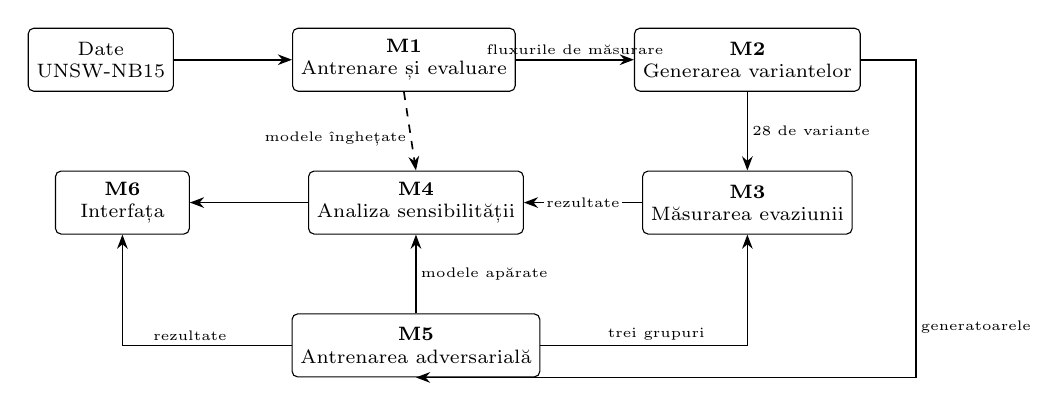
\begin{tikzpicture}[node distance=6mm and 15mm]
		\node[bloc, minimum width=17mm] (date) {Date\\ UNSW-NB15};
		\node[blocmare, right=of date] (m1) {\textbf{M1}\\ Antrenare și evaluare};
		\node[blocmare, right=of m1] (m2) {\textbf{M2}\\ Generarea variantelor};
		\node[blocmare, below=10mm of m2] (m3) {\textbf{M3}\\ Măsurarea evaziunii};
		\node[blocmare, left=of m3] (m4) {\textbf{M4}\\ Analiza sensibilității};
		\node[bloc, left=of m4, minimum width=17mm] (m6) {\textbf{M6}\\ Interfața};
		\node[blocmare, below=10mm of m4] (m5) {\textbf{M5}\\ Antrenarea adversarială};

		\draw[sageata] (date) -- (m1);
		\draw[sageata] (m1) -- node[eticheta, above] {fluxurile de măsurare} (m2);
		\draw[sageata] (m2) -- node[eticheta, right] {28 de variante} (m3);
		\draw[sageata] (m3) -- node[eticheta, midway, fill=white, inner sep=1pt] {rezultate} (m4);
		\draw[sageata] (m4) -- (m6);
		\draw[sageata] (m5.west) -| node[eticheta, pos=0.3, above] {rezultate} (m6.south);
		\draw[sageata] (m2.east) -- ++(7mm,0) |- node[eticheta, pos=0.42, right] {generatoarele} (m5.south);
		\draw[sageata] (m5.east) -| node[eticheta, pos=0.28, above] {trei grupuri} (m3.south);
		\draw[sageata] (m5.north) -- node[eticheta, right] {modele apărate} (m4.south);
		\draw[punctat] (m1.south) -- node[eticheta, pos=0.6, left] {modele înghețate} (m4.north);
	\end{tikzpicture}\\[1mm]
	{\footnotesize Structura funcțională a soluției. M4 se aplică de două ori, modelelor de
	referință și celor apărate. M6 este singurul modul terminal.}
\end{figure}

\section{Rezultate obținute}

\textbf{Vulnerabilitatea.} O singură modificare a valorii TTL, realizabilă prin configurarea
socketului, duce modelul cu cel mai bun macro-$F1$ de la $0\%$ la peste $50\%$ evaziune;
combinată cu umplutură și dilatare temporală, rata ajunge la aproape $97\%$. Celelalte
transformări lasă evaziunea sub $1{,}3\%$ la orice intensitate.

\textbf{Cauza.} Valoarea TTL este un artefact al mediului de captură, nu o proprietate a
atacurilor: în partiția de antrenare, $70{,}5\%$ din traficul legitim are valoarea 31, iar
fiecare clasă de atac are dominanta 254. Mărimea introdusă în lucrare, \emph{fracțiunea
accesibilă} $\rho$, arată că modelele se ordonează invers față de rezistența lor:
$84{,}1\%$ la XGBoost, $53{,}6\%$ la Random Forest, $26{,}0\%$ la Transformer. Rezistența
Transformer nu provine dintr-o reprezentare mai bună, ci din dependența de o caracteristică
generată de victimă.

\textbf{Apărarea.} Reantrenarea reduce evaziunea în cel mai rău caz sub $0{,}5\%$ la toate
trei modelele, de la valori între $71\%$ și $97\%$, iar câștigul se menține față de grupul de
control. Costul este sub $0{,}023$ de macro-$F1$, dar concentrat: clasa cea mai rară pierde
între $0{,}075$ și $0{,}127$. Analiza sensibilității aplicată modelelor apărate arată
\emph{prin ce} s-a obținut rezultatul: TTL-ul sursă cade de pe locul 1 pe locurile 38--41 din
42, iar $\rho$ scade la $7$--$19\%$. Modelele nu au memorat perturbările, au abandonat
caracteristica. Invarianța se transferă însă la o familie nevăzută doar la unul dintre cele
trei modele, iar dependența se mută pe TTL-ul de răspuns, tot un artefact de captură.

\section{Testări și verificări}

Validarea este organizată pe patru niveluri: determinism, validitate a variantelor, testare
negativă a suitei de validare și invarianți de capăt la capăt. Verificările executate:

\begin{itemize}
	\item varianta neperturbată reproduce predicțiile de referință rând cu rând, pe întreaga
	partiție de testare, și produce evaziune nulă;
	\item grupul de referință al antrenării adversariale reproduce modelele înghețate:
	0 nepotriviri din 82\,332 la toate cele trei familii, iar rețeaua coincide și pe
	traiectoria de optimizare, până la a patra zecimală;
	\item lanțul de măsurare al apărării reproduce toate cifrele publicate anterior, cu o
	abatere maximă de $0{,}0000$ puncte procentuale pe 28 de variante;
	\item eroarea reziduală a propagării dependențelor este de ordinul $10^{-15}$;
	\item mulțimea comună acoperă între $96{,}3\%$ și $99{,}3\%$ din fluxurile de atac, deci
	comparațiile nu se fac pe un rest îngust;
	\item suita respinge efectiv variante invalide construite intenționat.
\end{itemize}

\section{Contribuții personale}

Formularea mulțimii perturbărilor admisibile și mecanismul de propagare care o face
realizabilă. Tratarea explicită a caracteristicii nereconstituibile prin raportare sub formă
de interval. Introducerea fracțiunii accesibile $\rho$, care leagă cantitativ importanța
caracteristicilor de rata de evaziune, exprimându-le în aceleași unități. Protocolul
experimental al apărării, cu grup de control, ponderi înghețate, mulțime comună și criterii
pre-înregistrate. Grupul antrenat cu o familie exclusă deliberat, care a arătat că robustețea
obținută nu se generalizează. Aplicarea analizei de sensibilitate modelelor apărate, care a
stabilit mecanismul apărării. Implementarea de la zero a arhitecturii Transformer și a
interfeței interactive, construită din aceleași primitive validate ca experimentele
sistematice.

\section{Surse de documentare}

Lucrarea se sprijină pe 25 de referințe, grupate pe patru direcții. \textbf{Seturi de date:}
analiza comparativă a lui Ring et al., lucrarea de introducere a setului UNSW-NB15 a lui
Moustafa și Slay, CIC-IDS-2017, analiza critică a setului KDD CUP 99 și studiul lui Liu et
al. asupra erorilor din seturile CIC. \textbf{Modele de clasificare:} Breiman, Chen și
Guestrin, plus studii aplicate de detecție a intruziunilor. \textbf{Arhitecturi neuronale:}
lucrarea de referință a mecanismului de atenție, adaptarea la date tabulare a lui Gorishniy
et al., pe care se bazează implementarea, și lucrări de detecție bazate pe transformere.
\textbf{Învățare adversarială:} Szegedy et al. și Goodfellow et al. pentru originea
exemplelor adversariale, Madry et al. pentru formularea min-max a antrenării adversariale,
studii de evaziune specifice traficului de rețea și RFC~6274 pentru semantica câmpului TTL.

\end{document}
